\documentclass{article}
\usepackage{tikz}
\usetikzlibrary{calc,patterns,angles,quotes}
\begin{document}
  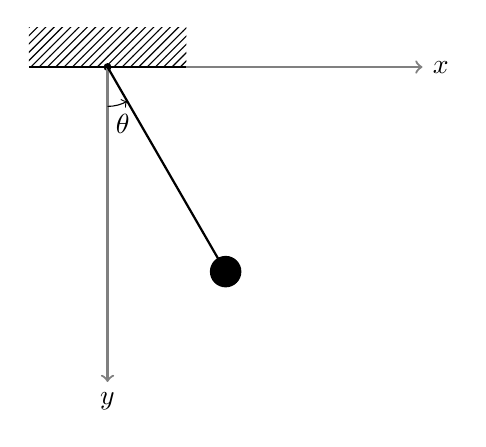
\begin{tikzpicture}
    \coordinate (origo) at (0,0);
    \coordinate (pivot) at (1,5);

    % draw axes
    \fill[black] (origo) circle (0.05);
    \draw[thick,gray,->] (origo) -- ++(4,0) node[black,right] {$x$};
    \draw[thick,gray,->] (origo) -- ++(0,-4) node (mary) [black,below] {$y$};

    % draw roof
    \fill[pattern = north east lines] ($ (origo) + (-1,0) $) rectangle ($ (origo) + (1,0.5) $);
    \draw[thick] ($ (origo) + (-1,0) $) -- ($ (origo) + (1,0) $);

    \draw[thick] (origo) -- ++(300:3) coordinate (bob);
    \fill (bob) circle (0.2);

    \pic [draw, ->, "$\theta$", angle eccentricity=1.5] {angle = mary--origo--bob};
  \end{tikzpicture}
\end{document}